% Vector composition; original audit package remains unchanged.
\begin{figure*}[!t]
\centering
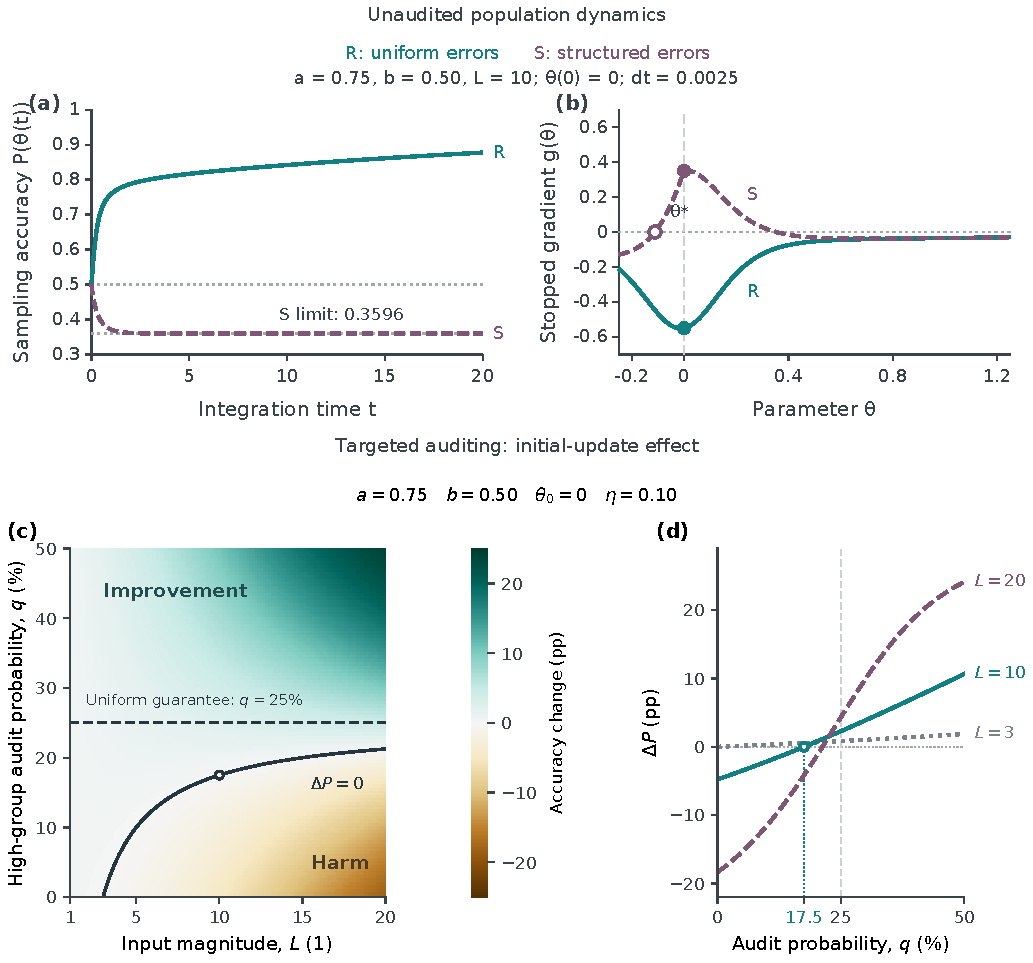
\includegraphics[width=0.6\textwidth]{figures/population_overview/population_overview.pdf}
\caption{Population dynamics and targeted auditing at $a=0.75$,
$b=0.5$, and $\theta_0=0$.
(a,b) Unaudited $R/S$ accuracy and gradients at $L=10$; filled/open
markers denote initial gradients/the negative $S$ equilibrium.
(c,d) Audited $S$ one-step change $100[P(-\eta g_{S,q}(0))-1/2]$ in
percentage points ($\eta=0.1$), with $L=3,10,20$ slices.
The solid boundary is $q_c(L)=0.25-0.75/L$ where nonnegative; the dashed
line marks the uniform flow threshold $q=0.25$ (Theorem~\ref{thm:audit}).
High-group query probability $q$ gives initial global query fraction
$B(q)=0.7q$. Panels (c,d) show initial updates, not convergence.
These are population calculations, not language-model measurements
(Appendix~\ref{app:numerical-readouts}).}
\label{fig:population-overview}
\end{figure*}
